% FRAME 1 
\section{Knot}
\begin{frame}{What is a knot}
	\centering
	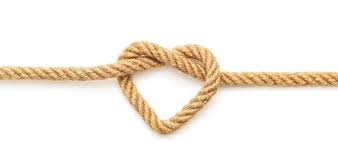
\includegraphics[width=7cm]{images/images.jpg}
	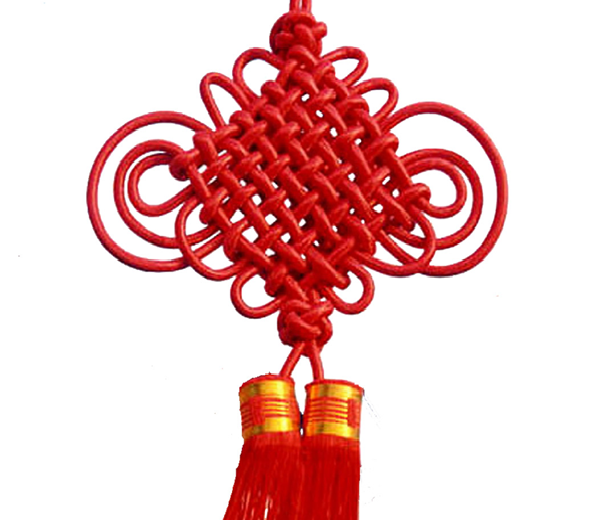
\includegraphics[width=3cm]{images/chineseknot.png}
\end{frame}

% FRAME 2 
\section{Knot}
\begin{frame}{What is a knot}
	\begin{itemize}
		\item To study knots rigorously, we need to connect the two ends of the rope.
	\end{itemize}
	\begin{kulblock}{Definition}
		In mathematics, a knot is an embedding of the circle $\mathbf{S}^1$ into 3-dimensional Euclidean space, $\mathbf{R}^3$.
	\end{kulblock}
	
\end{frame}

% FRAME 3
\begin{frame}{Motivation}
	\begin{itemize}
		\item Peter Guthrie Tait and Lord Kelvin (19th century): During the research on composition of atoms, they conjectured that atoms are made out of vortex ring of ether.
	\end{itemize}
	\centering
	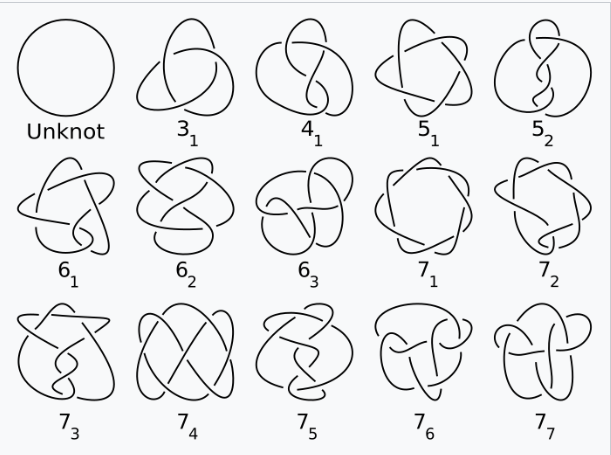
\includegraphics[width=5cm]{images/simple knots.png}
\end{frame}

% FRAME 4
\begin{frame}{Motivation}
	\begin{itemize}
		\item The structure of protein and DNA
	\end{itemize}
	\centering
	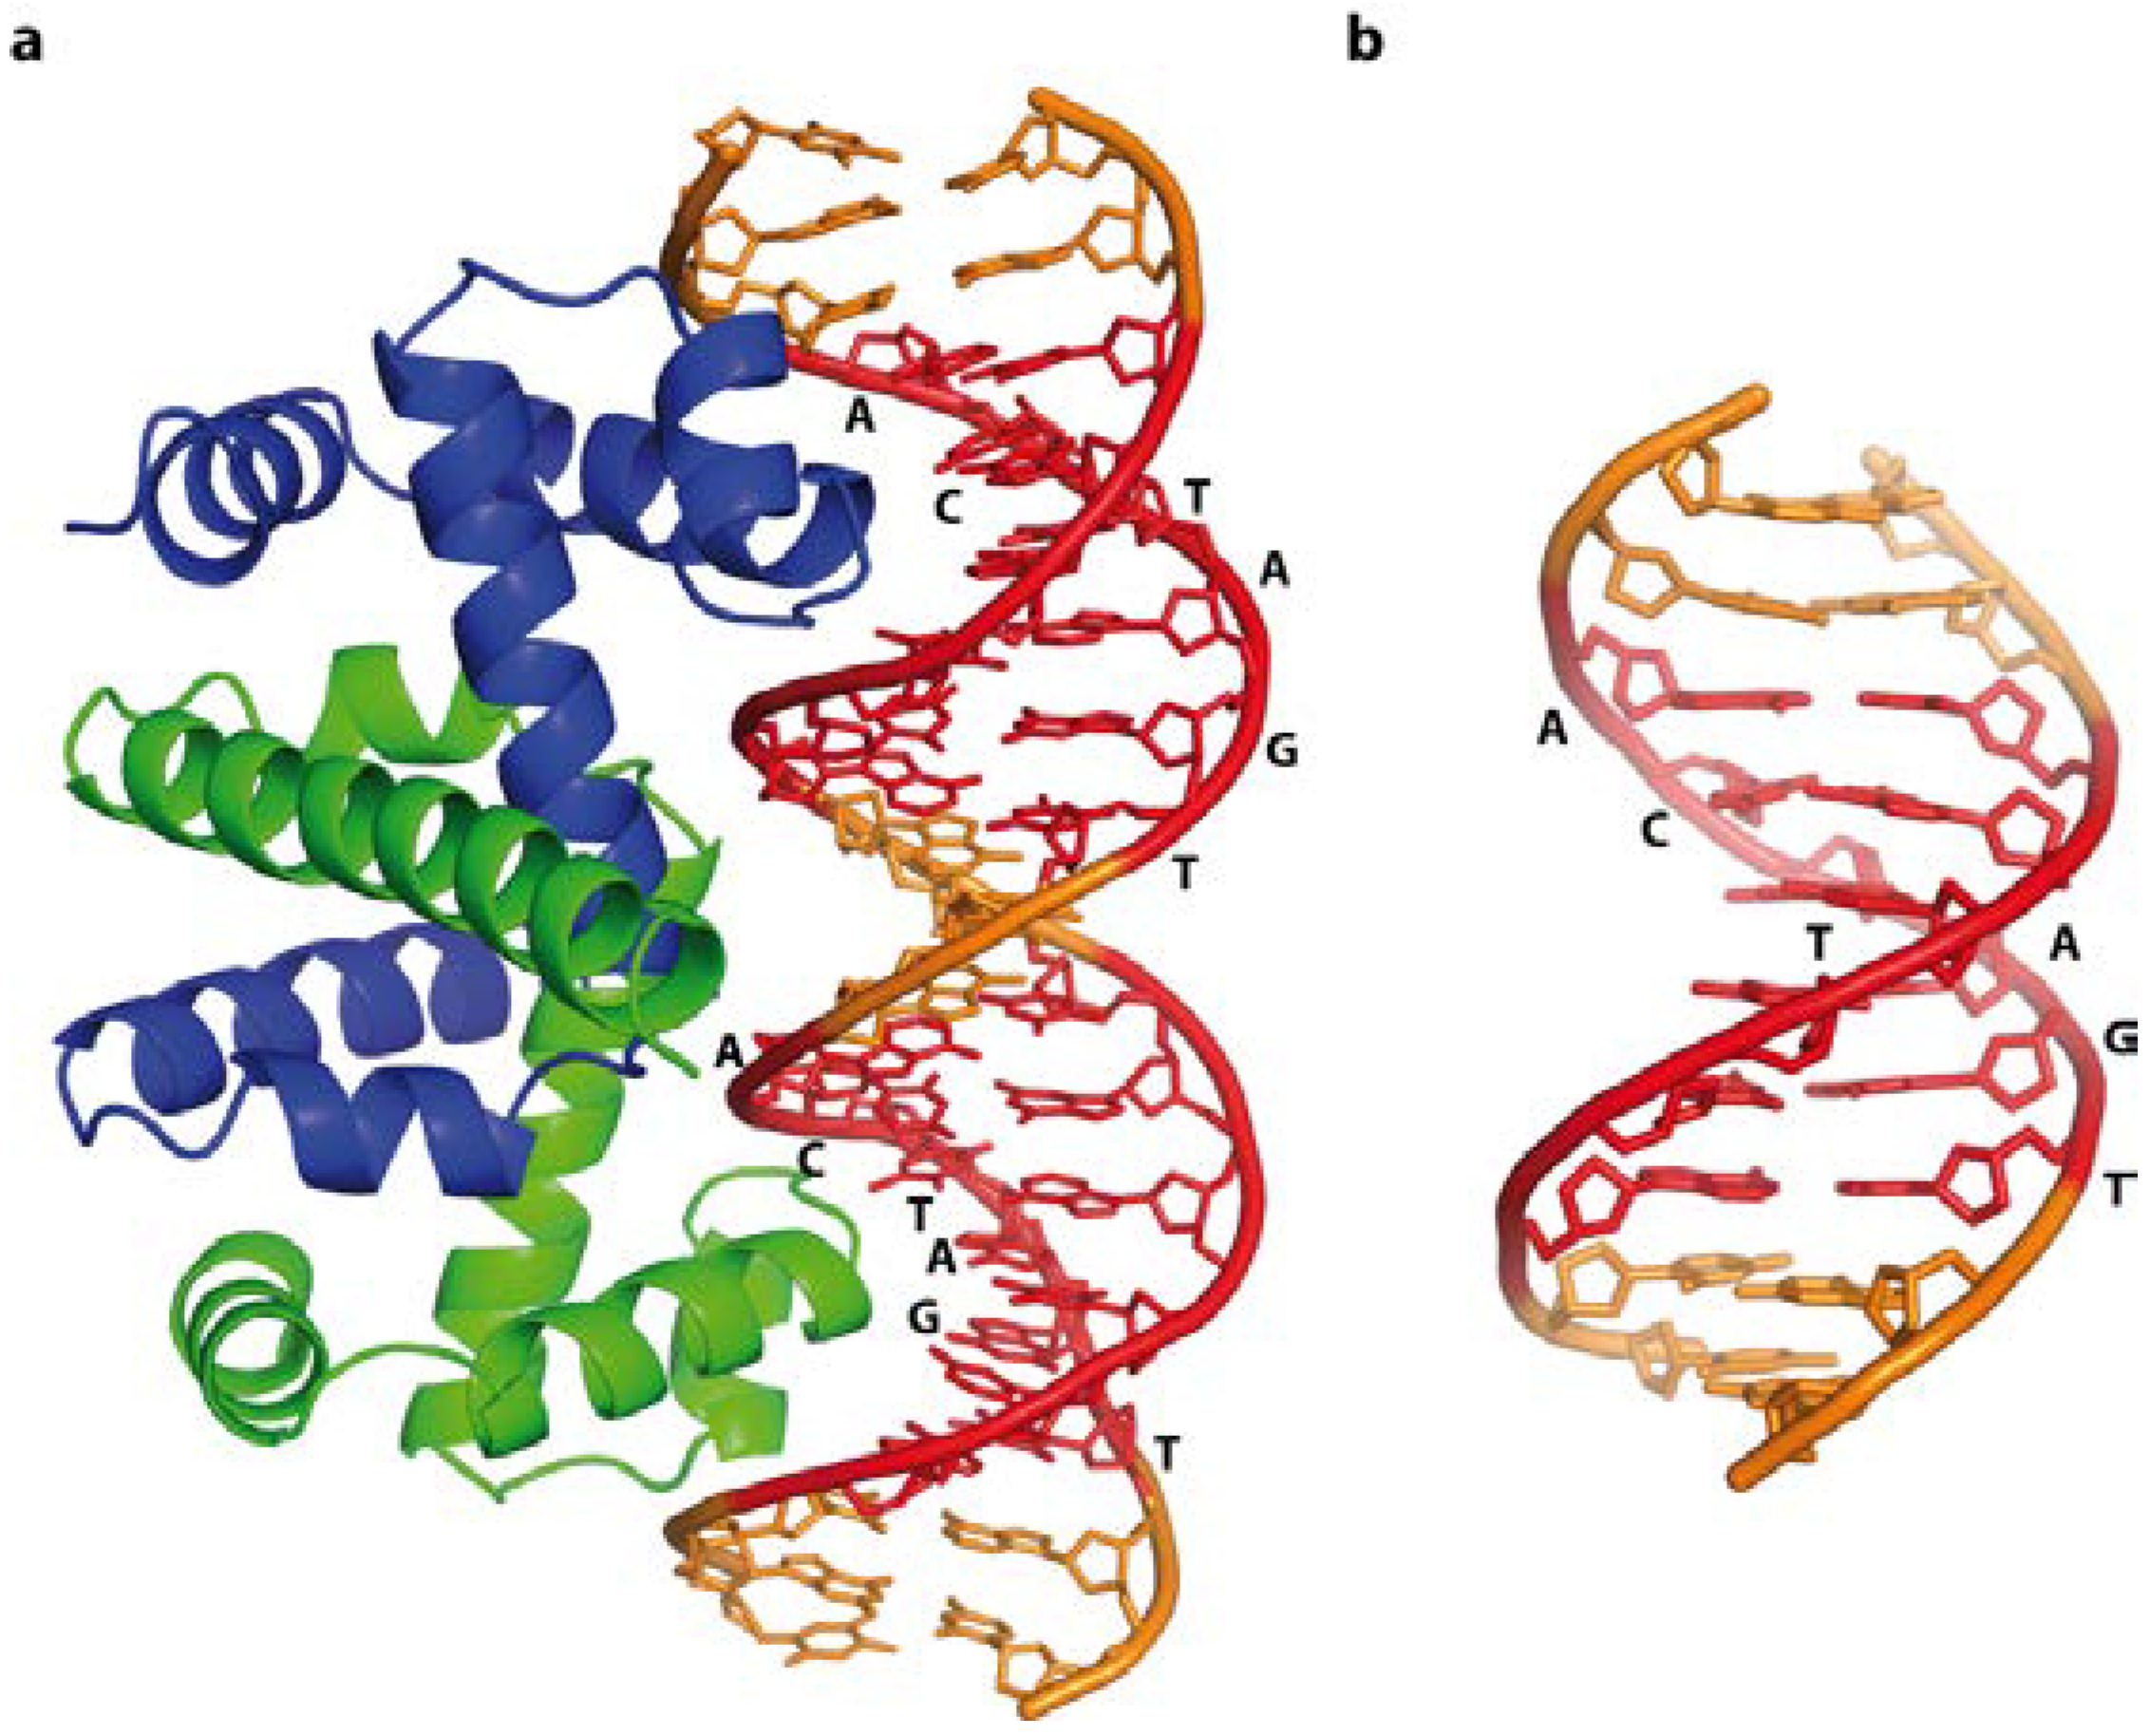
\includegraphics[width=7cm]{images/DNA.png}
\end{frame}

% FRAME 5
\begin{frame}{Motivation}
	\begin{itemize}
		\item The knot structure of material
	\end{itemize}
	\centering
	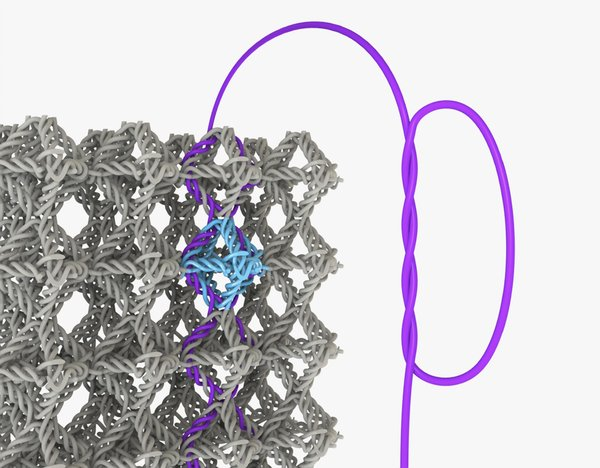
\includegraphics[width=7cm]{images/material.jpg}
\end{frame}

% FRAME 6
\begin{frame}{Diagram}
	\begin{itemize}
		\item How to represent a knot? Regular projection.
	\end{itemize}
	\begin{itemize}
		\item A knot projection is called a regular projection if no three points on the knot project to the same point, and no vertex
		projects to the same point as any other point on the knot.
	\end{itemize}
\end{frame}

% FRAME 7
\begin{frame}{Diagram}
	
	\begin{itemize}
		\item A knot diagram is the regular projection of a knot to the plane with broken
		lines indicating where one part of the knot undercrosses the other part.
	\end{itemize}
	\centering
	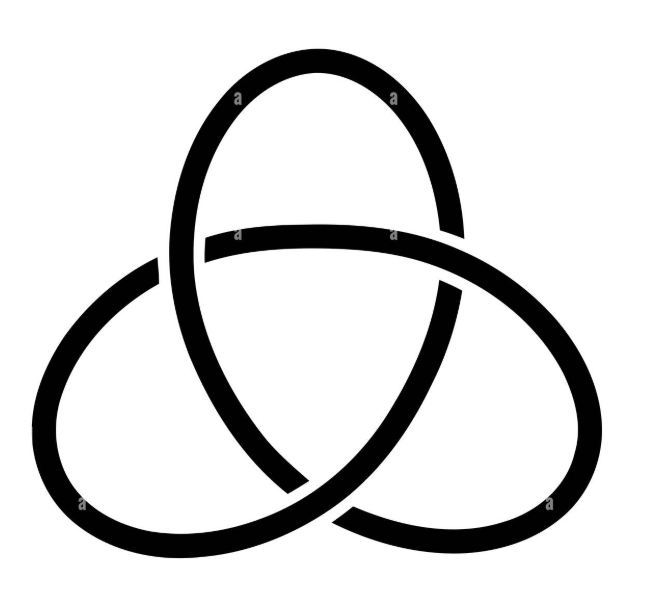
\includegraphics[width=3cm]{images/trefoil.png}
	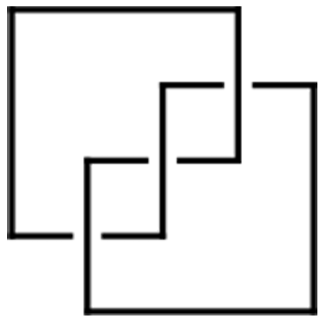
\includegraphics[width=3cm]{images/31.png}
\end{frame}

% FRAME 8
\begin{frame}{Reidemeister move}
	\begin{itemize}
		\item Equivalence of knot?
	\end{itemize}
	\centering
	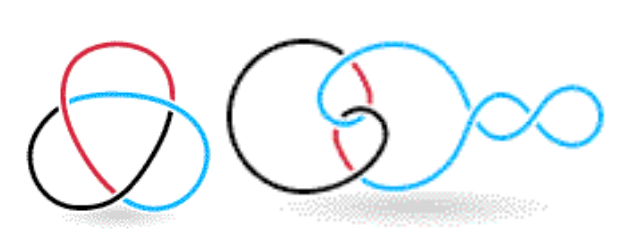
\includegraphics[width=7cm]{images/equivalence.png}
	
	\begin{itemize}
		\item Theorem: If two knots are equivalent, their diagrams are related by a sequence of Reidemeister moves.
	\end{itemize}
\end{frame}

% FRAME 9
\begin{frame}{Reidemeister move}
	\begin{itemize}
		\item A Reidemeister move is an operation that can be performed on the diagram
		of a knot whithout altering the corresponding knot.
	\end{itemize}
	\centering
	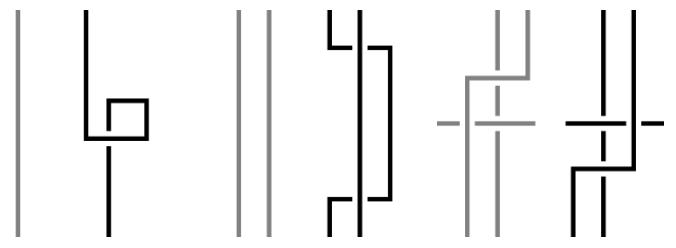
\includegraphics[width=7cm]{images/r.png}
\end{frame}